\section{MDA framework}

The MDA framework, used as a foundation for this work, is a widely accepted model for understanding and studying games, featuring over 1000 citations in April 2018 in google scholar. 

It's name is an acronym for Mechanics, Dynamics and Aesthetics, which are the three conceptual components games are made of. The framework also presents a causal relation between those components which is the most interesting contribution of this model. The MDA framework was created to help designers, scholars and researchers. Providing a tool for decomposing games in smaller parts, that are easier to manage and understand. 

The components of the framework are defined as \autoref{tab:MDA_components_description} illustrates:
{\renewcommand{\arraystretch}{1.5}
\begin{table}[!h]
    \caption{MDA components description \citep{Hunicke2004}}
    \vspace{.5em}
    \centering
    \begin{tabular}{c|m{6cm}l|}
    Mechanics &  The particular components of the games, at the level of data representation and algorithms.\\ \cline{1-2}
    Dynamics & The run-time behaviour of the mechanics, acting on player inputs and each others' outputs over time.\\ \cline{1-2} 
    Aesthetics & Emotional responses evoked in the players.\\
    \end{tabular}
    \label{tab:MDA_components_description}
\end{table}}


Those definitions, proposed by the authors, are fitting for the their model, but if we want to apply the model thoroughly in both game design and research. Deeper understanding of each of these concepts will be very useful. Hence this work intends to create an ontology for each of them, providing a tool that increases the usability of the MDA model for Boardgames. Even with a simple ontology and the foundations for a knowledge base, the use of each component of the MDA framework will be much clearer. As of today there is a lot of controversy about mechanics and aesthetics and for dynamics there is almost no information at all. With this work I intend to deliver not only a better  understanding of each component but also a coherent connection of their information to better serve the model.

%MDA diagram
\begin{figure}[ht]
\centering

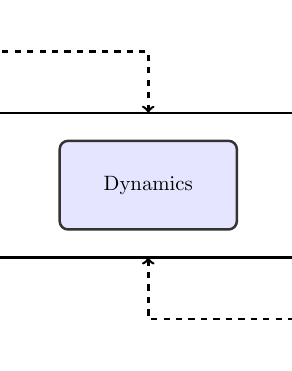
\begin{tikzpicture}[squarednode/.style={rectangle, 
					rounded corners, 
					very thick,
 					minimum width=3cm,
					minimum height=1.5cm,
					draw=black!80, 
					fill=green!10},
					squarednode2/.style={rectangle, 
					rounded corners, 
					very thick,
 					minimum width=3cm,
					minimum height=1.5cm,
					draw=black!80, 
					fill=blue!10},
					squarednode3/.style={rectangle, 
					rounded corners, 
					very thick,
 					minimum width=3cm,
					minimum height=1.5cm,
					draw=black!80, 
					fill=red!10}
					]
					
% To reduce all image, transform canvas
% forgets about image size, so 
% we need a bounding box
% This is lame, but works with Eduardo Thesis´s image (now black and white for elegance)

% don´t ask me about theses limits
% I just tried until I found which ones
%workded
\useasboundingbox (3,-2) rectangle (6,2);
\scope[transform canvas={scale=.75}]
         % Your actual drawing


%MDA nodes
\node[squarednode]  (m) [anchor = west]{Mechanics};
\node[squarednode2]  (d) [right of = m, node distance=3cm, anchor=west] {Dynamics};
\node[squarednode3]  (a) [right of = d, node distance=3cm, anchor=west] {Aesthetics};

%paths designer
%\path [-latex,  black, very thick] ([yshift=1ex]m.east) edge coordinate[midway](designerPath1) ([yshift=1ex]d.west);
%\path [-latex,  black, very thick] ([yshift=1ex]d.east) edge coordinate[midway](designerPath2) ([yshift=1ex]a.west);

% new designer path
\path[-latex, black, very thick] ([yshift=-3ex]a.south) edge  coordinate[midway](playerPathnew) ([yshift=-3ex]m.south);

%paths player
%\path [latex-, black, very thick] ([yshift=-1ex]m.east) edge  coordinate[midway](playerPath1)([yshift=-1ex]d.west);
%\path [latex-, black, very thick] ([yshift=-1ex]d.east) edge coordinate[midway](playerPath2) ([yshift=-1ex]a.west);

%new player path
\path[-latex, black, very thick] ([yshift=3ex]m.north) edge  coordinate[midway](designerPathnew) ([yshift=3ex]a.north);

%designer legend
\node [draw] (designerLegend) [above of = m, align=center, node distance=2cm, anchor=south]{\small Designer's Perspective};
\draw [dashed,<-,very thick](designerPathnew.north) |- (designerLegend.east);
%\draw [dashed,<-,very thick](designerPath2.north) |- (designerLegend.east);
%\draw [dashed,<-](designerPath2.north) |- (designerLegend.east);

%player legend
\node [draw] (playerLegend) [below of = a, align=center, node distance=2cm, anchor=north]{\small Player's Perspective};
%\draw[dashed, <-](playerPath1.south) |- (playerLegend.west);
\draw[dashed, <-,very thick](playerPathnew.south) |- (playerLegend.west);
%\draw[dashed, <-,very thick](playerPath1.south) |- (playerLegend.west);
    \endscope
\end{tikzpicture}
\caption{MDA diagram}
\label{fig:MDA_diagram}
\end{figure}

How each component of this model relates to each other can be understood through the diagram at \autoref{fig:MDA_diagram}. There are two agents of importance in this model, the player, who experiences the game and the designer who crafts the game each with a different perspective of the game. Those perspectives are of great importance to the MDA model, as they represent how the different agents involved in the game perceive it. 

The designer's perspective explains the reasoning used in the creation of the game, that is, how the design choices affect the game. Starting with the mechanics the designer chooses to include, he creates the artifact of the game. At this point the designer has full control of the artifact and knows exactly what is there and what is not. From the mechanics instanced in the game emerges dynamics, which depends on how the player will interact those mechanics. Because of this dependence the designer does not have the same power of control as with the mechanics, though it can still predicts what dynamics can appear with some level of accuracy. The farthest point from the designer is aesthetics which means it is the component the designer has least control. Representing the emotions experienced in gameplay, aesthetics are heavily dependent on the dynamics that happened in the game but even more from the player itself. Leaving the designer with just the expectation of what will happen in most cases, but not allowing the determination of a precise aesthetic response. 

The player's perspective addresses how the player experiences the game and how he interacts with each component of the game. The most important experience for the player is the aesthetic response it gets through playing a game. The player still has a certain responsibility for his aesthetics responses. He brings to the game his previous experiences, opinions and values, and is how they evaluate the gameplay that brings such responses. This is the component that has greater influence in the player judgment, it defines his opinions of the game, whether he likes it or not and how he feels about playing. Dynamics, to the player, is how gameplay develops, how he interact with other players and the game artifact. Such interaction is affected by the aesthetics experienced by the player throughout the gameplay and limited by the mechanics of the game. In mechanics the player withstand the set of rules and norms it has to oblige in order to play the game, in other words he sees them as the limitations and possibilities of the game. The player thus relates to the mechanics as a tool which allows him to interact with the game and as the rules that govern this interaction. 

 There is a practical example to illustrate such relationships. A said dynamic \textit{Run away} is an impulse created by the aesthetic \textit{Fear}, the player thus run because he is afraid. The player can only run because there is a mechanic \textit{Movement} that allows him to do so. At the same time this same movement mechanic could be used in a \textit{Charge} dynamic when it is related to the aesthetic of \textit{Fury}. It is important to note that such relations are not always reflective. In our example, run is caused by fear, but running does not inspire fear, another dynamic \textit{Find monster} is responsible to inspire this fear.
 
 \begin{figure}[h!]
     \centering 
     \includegraphics[scale = 0.55]{Images/MarioDiagram.png}
     \caption{Dynamics example}
     \label{fig:dynamicexample}
 \end{figure}

There is then a relationship between Mechanics and Dynamics as well as between Dynamics and Aesthetics that will feature in the boardgame ontology as relationships between the each particular ontology.